\nocite{*} %wszystkie wpisy trafią do bibliografii
\lstset{language=Java, tabsize=2,  basicstyle=\footnotesize\ttfamily, keywordstyle=\underbar}

% \setpagenumberingtype{gobble} % Remove page numbers (and reset to 1)
\setcounter{page}{1}
\newgeometry{tmargin=3cm, bmargin=3cm, lmargin=2cm, rmargin=2cm}

\newgeometry{tmargin=3cm, bmargin=3cm, lmargin=2cm, rmargin=2cm}

\thispagestyle {empty}

\begin{center}
	%logo uczelni
	
\includegraphics[scale=0.4]{img/pw}
	
	\vspace{0.5cm}
	
	{\fontsize{20}{20}\selectfont POLITECHNIKA WARSZAWSKA}
	
	\vspace{1.0cm}
	
	\textbf{{\fontsize{14}{14}\selectfont Wydział Mechatroniki}}
	
	\vspace{1.5cm}
	
	\textbf{{\fontsize{14}{14}\selectfont Praca magisterska}}

	\vspace{2.0cm}
	
	{\fontsize{14}{14}\selectfont Ireneusz Szulc}
	
	\vspace{1cm}
	
	{\fontsize{28}{28}\selectfont Planowanie bezkolizyjnych tras dla zespołu robotów mobilnych}
	
	\vspace{1cm}
	\begin{flushright}
		{\fontsize{14}{14}\selectfont Opiekun pracy: \\ 
		prof. nzw. dr hab. Barbara Siemiątkowska
		}
	
		\vspace{1cm}
		
		\vspace{3cm}
		% {\fontsize{14}{14}\selectfont Konsultant pracy: \\ 
		% mgr inż. }
		
	\end{flushright}
	
	\vspace{1cm}
	
	{\fontsize{12}{12}\selectfont Warszawa, 2018}
	
	%\cleardoublepage %nie działa
	
	%\clearpage\mbox{}\clearpage
\end{center}
\clearpage{\pagestyle{empty}\cleardoublepage}
\clearpage

\phantomsection
\addcontentsline{toc}{chapter}{Spis treści}
\tableofcontents
\clearpage

\raggedbottom
% \setpagenumberingtype{arabic} % kontynuowanie numerowania w stylu arabskim

\chapter{TODO}
\label{ch:todo}

Karta tematu: \\
Temat pracy: Planowanie bezkolizyjnych tras dla zespołu robotów mobilnych \\
Temat pracy (w jęz. ang.): Path planning for a group of mobile robots

Zakres pracy:
\begin{itemize}
	\item Projekt algorytmu wyznaczania trajektorii dla pojedynczego robota
	\item Algorytm detekcji i zapobiegania kolizjom między robotami
	\item Implementacja oprogramowania symulacyjnego
	\item Przeprowadzenie testów symulacyjnych
\end{itemize}

Podstawowe wymagania:
\begin{itemize}
	\item Aplikacja powinna umożliwiać symulację ruchu robotów oraz definiowanie położenia przeszkód przez użytkownika.
	\item Planowanie tras dotyczy robotów holonomicznych.
\end{itemize}

\chapter{Konspekt pracy}
\label{ch:konspekt}
\begin{itemize}
	\item Wstęp teoretyczny:
	\begin{itemize}
		\item Cooperative Pathfinding
		\item algorytm A* - szczegółowo
		\item przegląd metod planowania tras dla wielu robotów
		\item artykuł o Cooperative Pathfinding, time-space A*
		\item artykuł o wyznaczaniu priorytetów i metodach planowania tras (prezentacja): Path Coordination, time-space A*
		\item metoda ładunków - problem minimów lokalnych
		\item replanowanie po wykruciu kolizcji (algorytm D*)
		\item algorytmy WHCA* i IADPP
		\item Reciprocal Collision Avoidance
		\item metody przydziału priorytetów - zwiększanie i przeliczanie
		\item metody zcentralizowane vs rozproszone (porównanie)
		\item time-space A*, heurystyki, Reservation Table
	\end{itemize}
	\item zastosowanie: ciasne korytarze, częsty problem kolizji, szpitale, transport dokumentów, paczek
	\item generowanie mapy - labiryntu do testów: własny algorytm, teoria grafów, własności mapy
	\item time-space A* - pseudokod, schemat blokowy, własne heurystyki, modyfikacje
	\item metoda przydziału / zmiany priorytetów
	\item ograniczenia - nałożone uproszczenia: ruch skośny, czas dyskretny, brak czasu na obrót
	\item Implementacja aplikacji - stack technologiczny: Java 8, Java FX, Spring, Spring Boot, testy jednostkowe jUnit, git, IntelliJ, Maven, Linux; schemat klas aplikacji
	\item obszerne testy, porównanie wyników metod przy tych samych warunkacj początkowych
\end{itemize}
\clearpage{\pagestyle{empty}\cleardoublepage}

\chapter{Wstęp}
\label{ch:wstep}

\section{Cel pracy}
Przedmiotem niniejszej pracy jest przegląd metod rozwiązujacych zagadnienie planowania bezkolizyjnych tras dla wielu robotów. Stanowi to również wstęp teoretyczny do zaprojektowania algorytmu i implementacji oprogramowania pozwalającego na symulację działania systemu planowania tras.

Praca skupia się na przypadkach, w których mamy do czynienia ze środowiskiem z dużą liczbą przeszkód (np. zamknięty budynek z licznymi ciasnymi korytarzami), gdzie problem blokowania sią agentów prowadzi często do zakleszczenia. Należy wtedy zastosować nieco inne podejścia niż te, które sprawdzają się w przypadku otwartych środowisk, a które zostały opisane np. w pracach: \cite{roszkowska}, \cite{siemiatkowska}
$TODO$ W otwartych środowiskach mogą się dobrze sprawdzić D* albo LRA*

W niniejszej pracy zajmować będziemy się rozwiązaniem problemu, w którym mamy pełną informację o mapie otoczenia oraz o określonym położeniu początkowym i celu dla każdego z robotów. Zadaniem algorytmu będzie wyznaczenie możliwie najkrótszej bezkolizyjnej trasy dla wszystkich robotów. Należy jednak zaznaczyć, że priorytetem jest dotarcie każdego z robotów do celu bez kolizji z innymi robotami, dopiero później chcemy, aby wyznaczone drogi były możliwie najkrótsze.

$TODO$ zagadnienie z robotami holonomicznymi o zajętości przestrzennej równej 1 - nie mogą się mijać w tym samym korytarzu
Założenia pracy:
1. Planowanie tras dotyczy robotów holonomicznych.
2. Metody planowania powinny sprawdzać się w środowiskach z dużą liczbą przeszkód.
Zakres pracy:
1. Przegląd metod i algorytmów wykorzystywanych do koordynacji ruchu robotów.

$TODO$ bedzie to intro przez metody, aby dotrzeć wreszcie do WHCA*

\section{Koordynacja ruchu robotów}
Koordynacja ruchu robotów jest jednym z fundamentalnych problemów w systemach wielu robotów. \cite{optpriorities}

Kooperacyjne znajdowanie tras (ang. Cooperative Pathfinding) jest problemem planowania w układzie wieloagentowym, w którym to agenci mają za zadanie znaleźć bezkolizyjne drogi do swoich, osobnych celów. Planowanie to odbywa się w oparciu o pełną informację o środowisku oraz trasach pozostałych agentów. \cite{cooppath}

$TODO$ RTS - do skrótów
The interest in Multi-Agent Systems (MAS) is getting increased as more
complicated tasks has been introduced that can not be accomplished by a
single agent. Several domains have been built based on MAS, such as Real
Time Strategy (RTS) games 

Problem kooperacyjnego znajdowania tras pojawia się często m.in. w grach komputerowych, gdzie należy wyznaczyć drogi dla wielu jednostek, które mogą blokować się wzajemnie. Algorytmy do wyznaczania bezkolizyjnych tras dla wielu agentów (robotów) mogą znaleźć również zastosowanie w szpitalach (np. roboty TUG i HOMER do dostarczania sprzętu na wyposażeniu szpitala \cite{tughomer}) oraz magazynach (np. roboty transportowe w magazynach firmy Amazon \ref{fig:image_kiva_amazon}).

\begin{figure}[H]
	\centering
	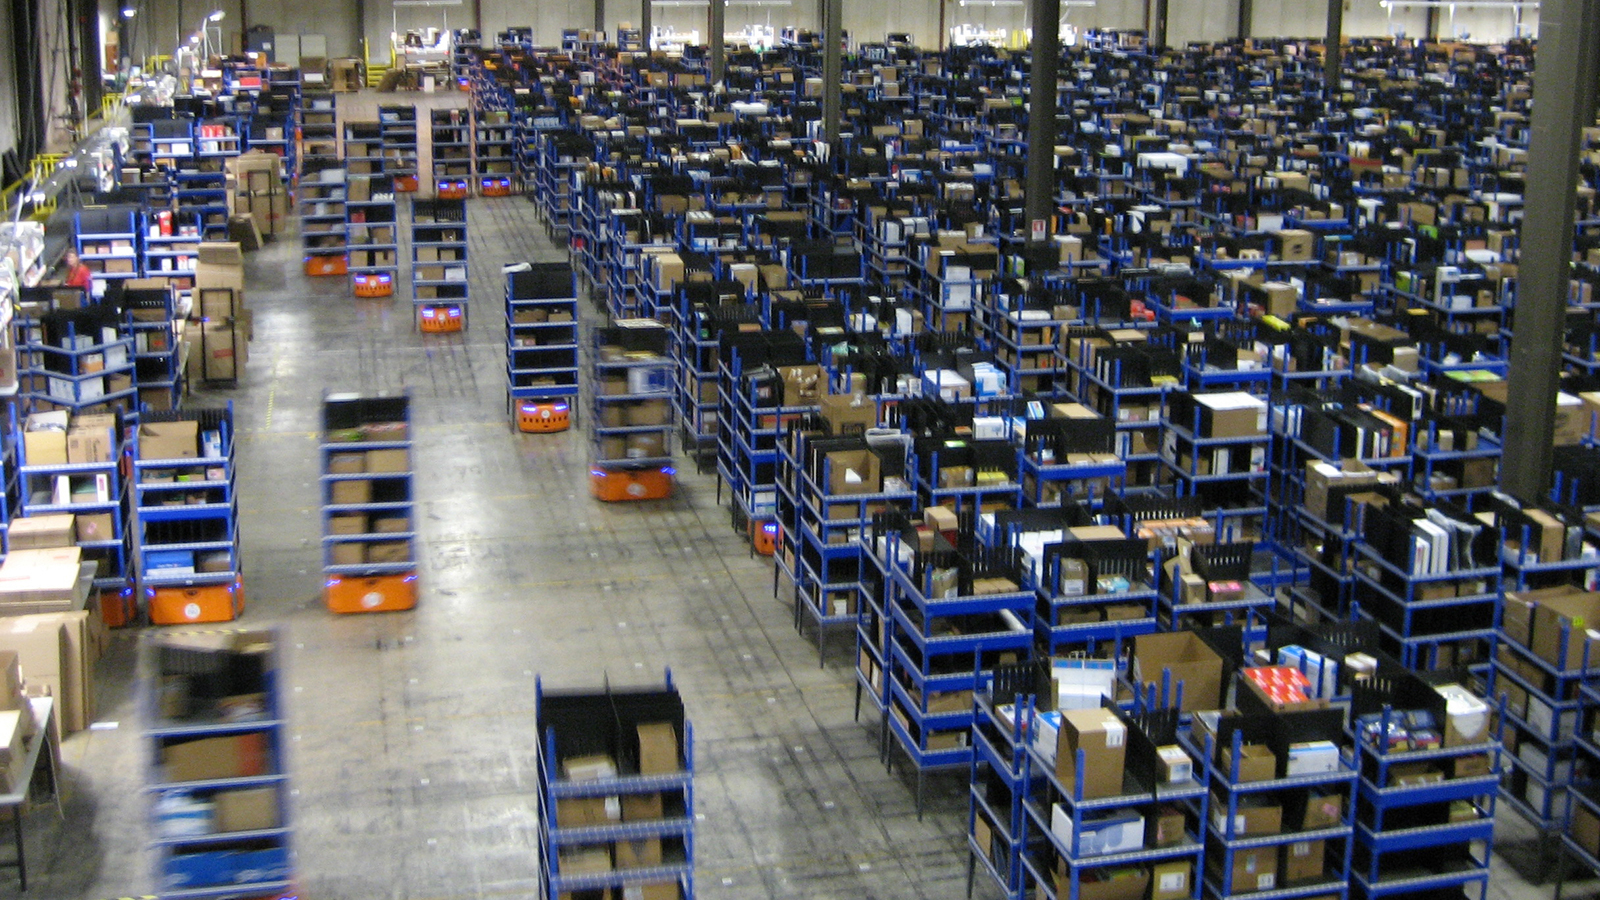
\includegraphics[width=14cm]{img/kiva-amazon}
	\caption{Roboty Kiva pracujące w magazynie firmy Amazon. Źródło: \cite{amazonkiva}}
	\label{fig:image_kiva_amazon}
\end{figure}

\section{Podstawowe pojęcia}
\subsubsection{Przestrzeń konfiguracyjna}
Przestrzeń konfiguracyjna to formalna, matematyczna przestrzeń będąca zbiorem możliwych stanów danego układu fizycznego.
W zależności od rodzaju i liczby wyróżnionych parametrów stanu przestrzenie konfiguracyjne mogą mieć wiele wymiarów.

\subsubsection{Robot holonomiczny}
$TODO$ dopisać definicje i uzupełnić w celu pracy, że będzie to ich dotyczyć

\subsubsection{Metoda hill-climbing}
$TODO$ wyjebać to?
Metoda hill-climbing jest rodzajem matematycznej optymalizacji, lokalną metodą przeszukiwania.
Jest to iteracyjny algorytm, który zaczyna w wybranym rozwiązaniu problemu, następnie próbuje znaleźć lepsze rozwiązanie poprzez przyrostowe zmiany pojedynczych elementów rozwiązania.
Jeśli zmiana przynosi lepsze rozwiązanie, jest wprowadzana do nowego rozwiązania.
Kroki algorytmu powtarzane są dotąd, aż żadne ``udoskonalenie'' nie zostaje znalezione.

\subsubsection{Zupełność algorytmu}
$TODO$

\chapter{Metody planowania tras}
\label{ch:path_planning_methods}

\section{Metody planowania tras}
$TODO$ wyjebać to gówno lub uogólnić
Spośród metod wykorzystywanych do planowania tras dla wielu robotów można wyróżnić dwie zasadnicze grupy \cite{latombe}:
$TODO$ zcentralizowanie nie muszą być optymalne
\begin{itemize}
	\item {\bf Zcentralizowane} - drogi wyznaczane są dla wszystkich agentów na raz (jednocześnie). Metody te potrafią znaleźć wszystkie możliwe rozwiązania (w szczególności to optymalne), ale mają bardzo dużą złożoność obliczeniową ze względu na ogromną przestrzeń przeszukiwania. Z tego powodu stosowane są heurystyki przyspieszające proces obliczania rozwiązania.
	\item {\bf Rozproszone} (ang. {\it decoupled} lub {\it distributed}) - Podejście to dekomponuje zadanie na niezależne lub zależne w niewielkim stopniu problemy dla każdego agenta. Dla każdego robota droga wyznaczana jest osobno, w określonej kolejności, następnie rozwiązywane są konflikty (kolizje dróg). W pewnych przypadkach rozwiązanie może nie zostać znalezione, mimo, iż istnieje. Zastosowanie metod rozproszonych wiąże się najczęściej z koniecznością przydzielenia priorytetów robotom, co stanowi istotny problem, gdyż od ich wyboru może zależeć zupełność algorytmu. Nie należy mylić tej metody z zagadnieniem typu {\it Non-Cooperative Pathfinding}, w którym agenci nie mają wiedzy na temat pozostałych planów i muszą przewidywać przyszłe ruchy pozostałych robotów \cite{cooppath}. W podejściu rozproszonym agenci mają pełną informację na temat stanu pozostałych robotów, lecz wyznaczanie dróg odbywa się w określonej kolejności.
\end{itemize}

$TODO$
- Plan all units simultaneously
	- Computationally intractable
	- $(units x actions)^depth$
- Plan individual units
	- Not complete
	- A lot of techniques needed to be practical

$TODO$
Dyskretna siatka pól - podział w celu szybszych obliczeń i wykorzystania A* (większość jest oparta na tym) - tak się stosuje w grach
$TODO$ - tutaj screen z warcraft map editora
Obrazek: Transform terrain to large grid [screenshot taken from Warcraft III map editor]. \cite{hierpathfindinginrts}
Use abstract maps to reduce computational costs
$TODO$ Pacman tu albo przy heurystykach
\begin{figure}[H]
	\centering
	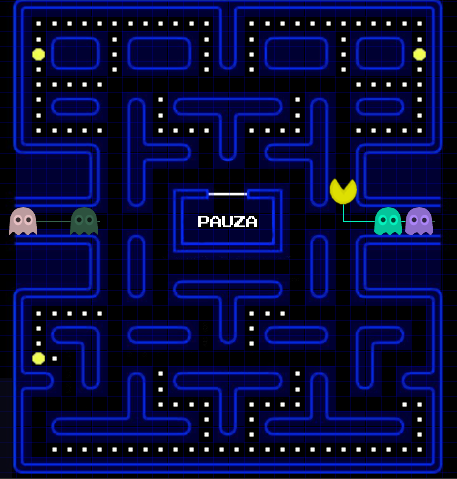
\includegraphics[width=13cm]{img/paclan1}
	\caption{Podział mapy na siatkę pól, zastosowanie heurystyki uwzględniającej zawijanie mapy po bokach, Źródło: własna implementacja gry}
	\label{fig:image_paclan1}
\end{figure}

\subsection{Metody zcentralizowane}
Wiele metod zcentralizowanych cechuje się planowaniem w zbiorowej przestrzeni konfiguracyjnej oraz możliwością wyznaczenia optymalnego rozwiązania.
Wadą jest natomiast duża złożoność obliczeniowa algorytmu i konieczność posiadania pełnej informacji o stanie otoczenia i robotów.

W systemach czasu rzeczywistego istotne jest, aby rozwiązanie problemu planowania tras uzyskać w określonym czasie, dlatego w tego typu sytemach częściej używane są techniki rozproszone.

$TODO$ Podejmowanie decyzji na podstawie centralnego systemu - scentralizowana struktura organizacyjna

\subsection{Metoda pól potencjałowych}
$TODO$ nie pisać, że to zcentralizowana, czy nie
Nie wszystkie podejścia zcentralizowane gwarantują optymalne rozwiązanie. Przykładem takiej metody, która nie daje gwarancji optymalności (ani nawet zupełności) jest metoda pól potencjałowych.

Metoda pól potencjałowych (ang. {\it Artificial Potential Field} lub {\it Potential Field Techniques}) polega na zastosowaniu zasad oddziaływania między ładunkami znanych z elektrostatyki. Roboty i przeszkody traktowane są jako ładunki jednoimienne, przez co "odpychają się" siłą odwrotnie proporcjonalną do kwadratu odległości (dzięki temu unikają kolizji między sobą). Natomiast punkt docelowy robota jest odwzorowany jako ładunek o przeciwnym biegunie, przez co robot jest "przyciągany" do celu.
Główną zasadę działania metody przedstawiono na rysunku \ref{fig:image_potentialfield}.
Technika ta jest bardzo prosta i nie wymaga wykonywania złożonych obliczeń (w odróżnieniu do pozostałych metod zcentralizowanych). Niestety bardzo powszechny jest problem osiągania minimum lokalnego, w którym suma wektorów daje zerową siłę wypadkową. Robot zostaje "uwięziony" w minimum lokalnym, przez co nie jest w stanie dotrzeć do wyznaczonego celu. Do omijania tego problemu muszą być stosowane inne dodatkowe metody. \cite{potentialfield}
\begin{figure}[H]
	\centering
	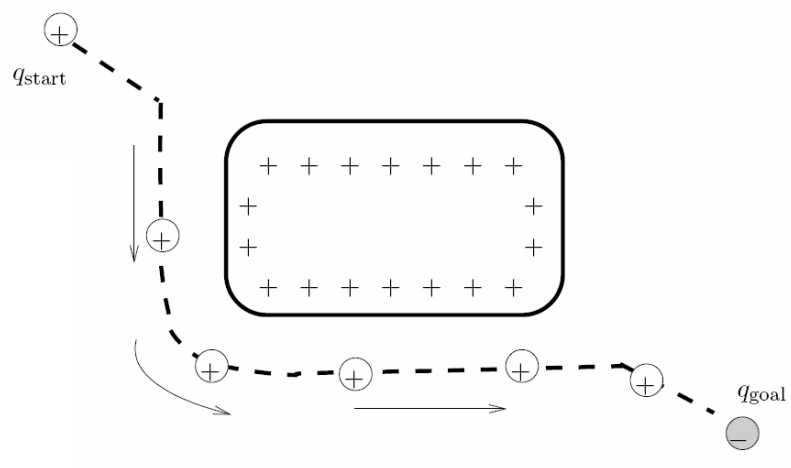
\includegraphics[width=12cm]{img/potential-field}
	\caption{Zasada działania metody pól potencjałowych. Źródło: \cite{howie_potentialfield}}
	\label{fig:image_potentialfield}
\end{figure}

\subsection{Rozproszone wyznaczanie tras}
$TODO$ wyjebać to gówno
Popularne podejścia unikające planowania w wysoko wymiarowej zbiorowej przestrzeni konfiguracyjnej to techniki rozproszone i priorytetowane.
Pomimo, że metody te są bardzo efektywne, mają dwie główne wady:
\begin{enumerate}
	\item Nie są zupełne - czasami nie udaje się znaleźć rozwiązania, nawet gdy istnieje.
	\item Wynikowe rozwiązania są często nieoptymalne.
\end{enumerate}

W artykule \cite{optpriorities} przedstawione zostało podejście do optymalizowania układu priorytetów dla rozproszonych i priorytetowanych technik planowania.
Proponowana metoda wykonuje randomizowane przeszukiwanie z techniką hill-climbing do znalezienia rozwiązania i do skrócenia całkowitej długości ścieżek.
Technika ta została zaimplemenotwana i przetestowana na prawdziwych robotach oraz w rozległych testach symulacyjnych.
Wyniki eksperyentu pokazały, że metoda potrafi znacząco zmniejszyć liczbę niepowodzeń i znacznie zmniejszyć całkowitą długość tras dla różnych priorytetowanych i rozproszoncyh metod planowania dróg, nawet dla dużych zespołów robotów.

Najczęściej stosowanymi podejściami są metody oparte o algorytm A*. W szczególności są to:
\begin{itemize}
	\item A* w konfiguracji czaso-przestrzennej
	\item Path coordination
\end{itemize}

\subsubsection{Path coordination}
Idea metody Path coordination przedstawia się następująco \cite{optpriorities}:
\begin{enumerate}
	\item Wyznaczenie ścieżki dla każdego robota {\bf niezależnie}
	\item Przydział priorytetów
	\item Próba rozwiązania możliwych konfliktów między ścieżkami. Roboty utrzymywane są na ich indywidualnych ścieżkach (wyznaczonych na początku), wprowadzane modyfikacje pozwalają na zatrzymanie się, ruch naprzód, a nawet cofanie się, ale tylko {\bf wzdłuż trajektorii} w celu uniknięcia kolizji z robotem o wyższym priorytecie.
\end{enumerate}
Złożoność metody wynosi $O(n \cdot m \cdot log(m))$, $m$ - maksymalna liczba stanów podczas planowania, $n$ - liczba robotów


\subsection{Priorytetowane planowanie}
$TODO$
In general, the complexity of complete approaches to multi-agent
path planning grows exponentially with the number of agents. There-
fore, the complete approaches often do not scale-up well and hence
are often not applicable for nontrivial domains with many agents. To
plan paths for a high number of agents in a complex environment,
one has to resort to one of the incomplete, but fast approaches. A
simple method often used in practice is prioritized planning [3, 9, 1].
In prioritized planning the agents are assigned a unique priority. In
its simplest form, the algorithm proceeds sequentially and agents
plan individually from the highest priority agent to the lowest one.
The agents consider the trajectories of higher priority agents as con-
straints (moving obstacles), which they need to avoid. It is straight-
forward to see that when the algorithm finishes, each agent is as-
signed a trajectory not colliding with either higher priority agents,
since the agent avoided a collision with those, nor with lower priority
agents who avoided a conflict with the given trajectory themselves.

The complexity of the generic algorithm grows linearly with the
number of agents, which makes the approach applicable for problems
involving many agents. Clearly, the algorithm is greedy and incom-
plete in the sense that agents are satisfied with the first trajectory not
colliding with higher priority agents and if a single agent is unable to
find a collision-free path for itself, the overall path finding algorithm
fails. The benefit, however, is fast runtime in relatively uncluttered
environments, which is often the case in multi-robotic applications.
Prioritized planner is also sensitive to the initial prioritization of the
agents. Both phenomena are illustrated in Figure 1 that shows a sim-
ple scenario with two agents desiring to move from s1 to d1 (s2 to d2
resp.) in a corridor that is only slightly wider than a single agent. The
scenario assumes that both agents have identical maximum speeds.
\cite{async_decentralized_spacetime_cp}


\begin{figure}[H]
	\centering
	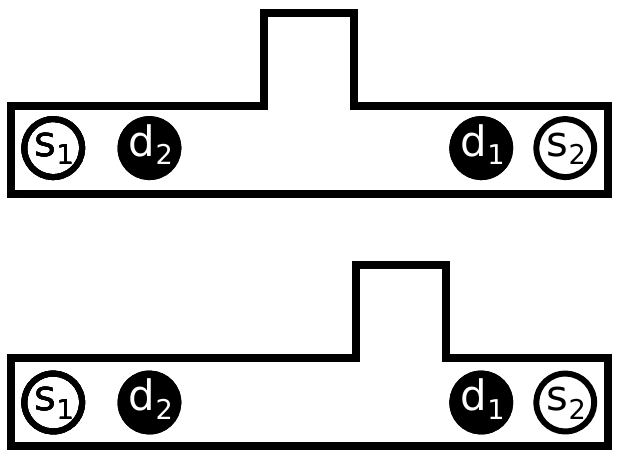
\includegraphics[width=10cm]{img/prioritized-planning-problem1}
	\caption{Top: example of a problem to which a prioritized planner
will not find a solution. The first agent plans its optimal path first,
but such a trajectory is in conflict with all feasible trajectories of the
second agent. Bottom: example of a problem to which a prioritized
planner will find a solution only if agent 1 has a higher priority than
agent 2. Źródło: \cite{async_decentralized_spacetime_cp}}
	\label{fig:img_prioritized-planning-problem1}
\end{figure}

\subsection{Wybór priorytetów}
$TODO$ nie dotyczy tylko Path coordination, ale też A* time-space
Istotną rolę doboru priorytetów robotów w procesie planowania tras ukazuje prosty przykład przedstawiony na rysunku \ref{fig:image_article1_fig1}. Jeśli robot 1 (zmierzający z punktu S1 do G1) otrzyma wyższy priorytet niż robot 2 (zmierzający z S2 do G2), spowoduje to zablokowanie przejazdu dla robota 2 i w efekcie prawidłowe rozwiązanie nie zostanie znalezione.
\begin{figure}[H]
	\centering
	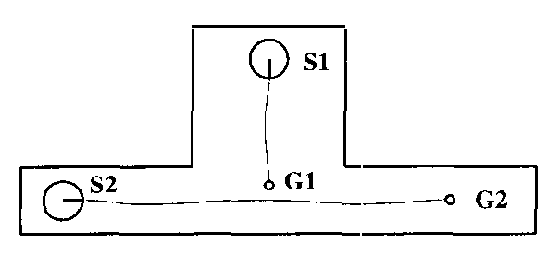
\includegraphics[width=10cm]{img/article1/fig1}
	\caption{Sytuacja, w której żadne rozwiązanie nie zostanie znalezione, jeśli robot 1 ma wyższy priorytet niż robot 2. Źródło: \cite{optpriorities}}
	\label{fig:image_article1_fig1}
\end{figure}

Układ priorytetów może mieć również zasadniczy wpływ na długość uzyskanych tras. Odpowiedni przykład został przedstawiony na rysunku \ref{fig:image_article1_ppt6}. W zależności od wyboru priorytetów, wpływających na kolejność planowania tras, otrzymujemy różne rozwiązania.
\begin{figure}[H]
	\centering
	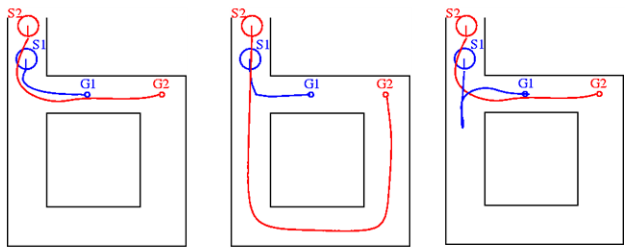
\includegraphics[width=13cm]{img/article1/ppt6}
	\caption{a) Niezależne planowanie optymalnych tras dla 2 robotów; b) suboptymalne rozwiązanie, gdy robot 1 ma wyższy priorytet; c) rozwiązanie, gdy robot 2 ma wyższy priorytet}
	\label{fig:image_article1_ppt6}
\end{figure}

\clearpage{\pagestyle{empty}\cleardoublepage}

\chapter{Algorytmy oparte o A*}
\label{ch:astar}

Kiedy pojedynczy agent dokonuje znalezienia drogi do wyznaczonego celu, prosty algorytm A* sprawdza się bardzo dobrze. Jednak w przypadku, gdy wiele agentów porusza się w tym samym czasie, to podejście może się nie sprawdzić, powodując wzajemne blokowanie się i zakleszczenie jednostek. Rozwiązaniem tego problemu może być kooperacyjne znajdowanie tras. Roboty będą mogły skutecznie przemieszczać się przez mapę, omijając trasy wyznaczone przez inne jednostki oraz schodząc innym jednostkom z drogi, jeśli to konieczne. \cite{cooppath}

Zagadnienie znajdowania drogi jest ważnym elementem sztucznej inteligencji zaimplementowanej w wielu grach komputerowych. Chociaż klasyczny algorytm A* potrafi doprowadzić pojedynczego agenta do celu, to jednak dla wielu agentów wymagane jest zastosowanie innego podejścia w celu unikania kolizji. Algorytm A* może zostać zaadaptowany do replanowania trasy na żądanie, w przypadku wykrycia kolizji tras (Local Repair A* lub D*). Jednak takie podejście nie jest zadowalające pod wieloma względami. Na trudnych mapach z wieloma wąskimi korytarzami i wieloma agentami może to prowadzić do zakleszczenia agentów w wąskich gardłach lub do cyklicznego zapętlenia ruchu agentów. \cite{cooppath}

$TODO$ Które algorytmy tylko znajdują droge, a które rozwiązują problem kolizji

$TODO$ Większość z tych algorytmów wykorzystywana jest w grach. planowanie musi odbywać się szybko, szczególnie w grach (screen warcraft :))

\section{Algorytm A*}
A* jest algorytmem heurystycznym służącym do przeszukiwania grafu w celu znalezienia najkrótszej ścieżki. Algorytm ten jest powszechnie stosowany w zagadnieniach sztucznej inteligencji oraz w grach komputerowych \cite{mit_astar}. Jest modyfikacją algorytmu Dijkstry, wprowadza pojęcie funkcji heurystycznej $h(n)$. Wartość funkcji heurystycznej powinna określać przewidywaną drogę do węzła docelowego. W każdym kroku przeszukiwany jest węzeł o najmniejszej wartości funkcji $f(n)$.

\begin{gather}
 	f(n) = g(n) + h(n)
 	\label{eq_astar} 
\end{gather}
 gdzie:

 $g(n)$ - wartość kosztu, dokładna odgległość miedzy węzłem $n$ a węzłęm startowym

 $h(n)$ - heurystyka, przewidywana droga do węzła docelowego

 $n$ - węzeł, wierzchołek przeszukiwanego grafu

Dzięki takiemu podejściu najpierw sprawdzane są najbardziej "obiecujące" rozwiązania, co pozwala szybciej otrzymać rozwiązanie (w przeciwieństwie do algorytmu Dijkstry).
Algorytm kończy działanie w momencie, gdy napotka węzeł będący węzłem docelowym.
Dla każdego odwiedzonego węzła zapamiętywane są wartości $g(n)$, $h(n)$ oraz węzeł będący rodzicem w celu późniejszego odnalezienia drogi powrotnej do węzła startowego po napotkaniu węzła docelowego (por. rys. \ref{fig:image_astar2}).

\begin{figure}[H]
	\centering
	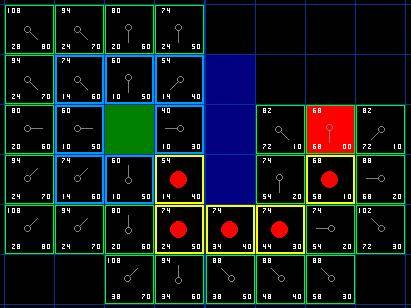
\includegraphics[width=10cm]{img/astar-t7}
	\caption{Przykład działania algorytmu A*. Źródło: \cite{astar2}}
	\label{fig:image_astar2}
\end{figure}

\subsection{Heurystyki}
Od wyboru sposobu obliczania heurystyki zależy czas wykonywania algorytmu oraz optymalność wyznaczonego rozwiązania.
Poniżej przedstawiono najczęściej wykorzystywane heurystyki.

$TODO$ Jeśli wartość heurystyki <= od rzeczywistej drogi, jaka musi zostać przebyta, to wyznaczona scieżka jest ścieżką optymalną (najkrótszą)
= admissible heuristic
An admissible heuristic never overestimates the distance to the goal. A* search with an
admissible heuristic is guaranteed to find the shortest path. However, there is a stronger
property, known as consistency [Russell03]. A consistent heuristic maintains the property
h(A) ≤ cost(A, B) + h(B) between all locations A and B. In other words, the estimated
distance doesn’t jump around between the locations along a path.
\cite{cooppath}

A* opiera się na heurystyce, która prowadzi przeszukiwaniem. Słaba heurystyka może prowadzić do zbędnego odwiedzania dodatkowych węzłów.

\subsubsection{Heurystyka Euklidesowa}
Dla dwuwymiarowej mapy heurystyka euklidesowa wyraża dokładną odległość między przeszukiwanym węzłem $(x_n, y_n)$ a węzłem docelowym $(x_g, y_g)$:
\begin{gather}
 	h(n) = \sqrt{(x_n - x_g)^2 + (y_n - y_g)^2}
 	\label{eq_astar_heu_euc} 
\end{gather}

\subsubsection{Heurystyka Manhattan}
W przypadku, gdy robot może poruszać się po mapie jedynie poziomo lub pionowo (nie na ukos) wystarczającym przybliżeniem jest metryka Manhattan:
\begin{gather}
 	h(n) = |x_n - x_g| + |y_n - y_g|
 	\label{eq_astar_heu_man} 
\end{gather}

$TODO$ Przykład z Pacmanem - screen - siatka podzielona na pola
zbliżenie do 0 sprowadza ją do ścieżki optymalnej (Dijkstry) - połowa heurystyki Manhattan daje możliwość wyznaczania trasy z uwzględnieniem zawijania mapy
The Manhattan distance is a consistent heuristic. The true distance heuristic is also consistent. (no chyba że zawijanie mapy)

\subsubsection{Heurystyka zerowa}
Przyjęcie heurystyki równej $h(n) = 0$ powoduje, że algorytm A* sprowadza się do algorytmu Dijkstry.

\section{Local Repair A*}
W algorytmie Local Repair A* (LRA*) każdy z agentów znajduje drogę do celu, używając algorytmu A*, ignorując pozostałe roboty oprócz ich obecnych sąsiadów. Roboty zaczynają podążać wyznaczonymi ścieżkami do momentu, aż kolizja z innym robotem jest nieuchronna. Wtedy następuje ponowne przeliczenie drogi pozostałej do przebycia, z uwzględnieniem nowo napotkanej przeszkody.

Możliwe (i całkiem powszechne \cite{cooppath}) jest uzyskanie cykli (tych samych sekwencji ruchów powtarzających się w nieskończoność), dlatego zazwyczaj wprowadzane są pewne modyfikacje, aby rozwiązać ten problem. Jedną z możliwości jest zwiększanie wpływu losowego szumu na wartość heurystyki. Kiedy agenci zachowują się bardziej losowo, prawdopodobne jest, że wydostaną się z problematycznego położenia i spróbują podążać innymi ścieżkami.

Algorytm ten ma jednak sporo poważnych wad, które szczególnie ujawniają się w trudnych środowiskach z dużą liczbą przeszkód. Wydostanie się z zatłoczonego wąskiego gardła może trwać bardzo długo. Prowadzi to również do ponownego przeliczania trasy w prawie każdym kroku. Wciąż możliwe jest również odwiedzanie tych samych lokalizacji w wyniku zapętleń.

$TODO$ Jest to przykład rozproszonej struktury organizacyjnej - Podejmowanie decyzji przez roboty lokalnie (+ centralnie)???

\section{Algorytm D*}
D* ({\it Dynamic A* Search}) jest przyrostowym algorytmem przeszukiwania. Jest modyfikacją algorytmu A* pozwalającą na szybsze replanowanie trasy w wyniku zmiany otoczenia (np. zajmowania wolnego pola przez innego robota). Wykorzystywany jest m.in. w nawigacji robota do określonego celu w nieznanym terenie. Początkowo robot planuje drogę na podstawie pewnych założeń (np. nieznany teren nie zawiera przeszkód). Podążając wyznaczoną ścieżką, robot odkrywa rzeczywisty stan mapy i jeśli to konieczne, wykonuje ponowne planowanie trasy na podstawie nowych informacji.
Często wykorzystywaną implementacją (z uwagi na zoptymalizowaną złożoność obliczeniową) jest wariant algorytmu {\it D* Lite} \cite{dstarlite}.

\section{Cooperative A*}
$TODO$
Cooperative A* jest algorytmem do rozwiązywania problemu kooperacyjnego znajdowania tras.
Metoda może być również nazywana czasoprzestrzennym algorytmem A* ({\it time-space A* search})
Zadanie planowania jest rozdzielone na serię pojedynczych poszukiwań dla poszczególnych agentów.
Pojedyncze poszukiwania są wykonywane w trójwymiarowej czasoprzestrzeni i biorą pod uwagę zaplanowane ścieżki przez pozostałych agentów.
Akcja wykonania postoju (pozostania w tym samym miejscu) jest uwzględniona w zbiorze akcji możliwych do wykonania.
Po przeliczeniu dróg dla każdego agenta, stany zajętości pól są zaznaczane w tablicy rezerwazji (ang. Reservation table).
Pozycje w tej tablicy są uważane jako pola nieprzejezdne i w efekcie są omijane podczas przeszukiwania przez późniejszych agentów. \cite{cooppath}

Należy zaznaczyć, że planowanie dla każdego agenta odbywa się sekwencyjnie według przydzielonych priorytetów.
Algorytm ten jest podatny na zmianę kolejności agentów. Odpowiedni dobór priorytetów może wpłynąć na wydajność algorytmu oraz jakość uzyskanego wyniku.

\subsection{Trzeci wymiar}
$TODO$
Do rozwiązania problemu kooperacyjnego znajdowania dróg algorytm przeszukiwania potrzebuje mieć pełną wiedzę na temat przeszkód oraz jednostek na mapie.
Aby zapisać tą informację potrzeba rozszerzyć mapę o trzeci wymiar - czas. 
Pierwotną mapę będziemy nazywac mapą przestrzenną, natomiast nową - czasoprzestrzenną mapą. \cite{cooppath}

Zagadnienie sprowadza się do przeszukiwania grafu, w którym każdy węzeł ma przypisane 3 wielkości: położenie x, położenie y oraz czas.
Podczas gdy zakres wielkości x i y jest znany i wynika z rozmiarów mapy oraz podziału jej wymiarów na dyskretne pola, to jednak określenie wymiaru czasu może być trudnym zagadnieniem.
Wymiar czasu możemy również zdyskretyzować i przyjać, że najmniejsza jednostka jest czasem, jaki zajmuje robotowi przejście z jednego pola na sąsiednie (poziomo lub pionowo). Natomiast górną granicą czasu powinna być maksymalna liczba ruchów potrzebna do dotarcia do celu przez ostatniego robota. Wybór za małej liczby może spowodować, że algorytm nie znajdzie drogi dla niektórych agentów, z kolei za duża granica czasu mocno wydłuża czas obliczeń. Rozwiązanie tego problemu zostało opisane w późniejszym podrozdziale \ref{ch:hier_cooperative_a}.

Wprowadzenie trzeciego wymiaru powoduje również konieczność zmian w doborze odpowiedniej heurystyki odpowiedzialnej za oszacowanie drogi pozostałej do celu.

\subsection{Tablica rezerwacji}
Tablica rezerwacji (ang. {\it Reservation Table}) reprezentuje wspódzieloną wiedzę o zaplanowanych ścieżkach przez wszystkich agentów.
Jest to informacja o zajętości każdej z komórki na mapie w danym miejscu i określonym czasie. \cite{cooppath}

Jak tylko agent zaplanuje trasę, każda komórka odpowiadająca ścieżce zaznaczana jest jako zajęta w tablicy rezerwacji.

W prostej implementacji tablica rezerwacji jest trójwymiarową kostką (dwa wymiary przestrzenne i jeden wymiar czasu).
Każda komórka kostki, która jest przecinana przez zaplanowaną przez agenta ścieżkę, jest zaznaczana jako nieprzejezdna przez określony czas trwania. W ten sposób zapobiega to planowania kolizyjnych tras przez pozostałych agentów.

\begin{figure}[H]
	\centering
	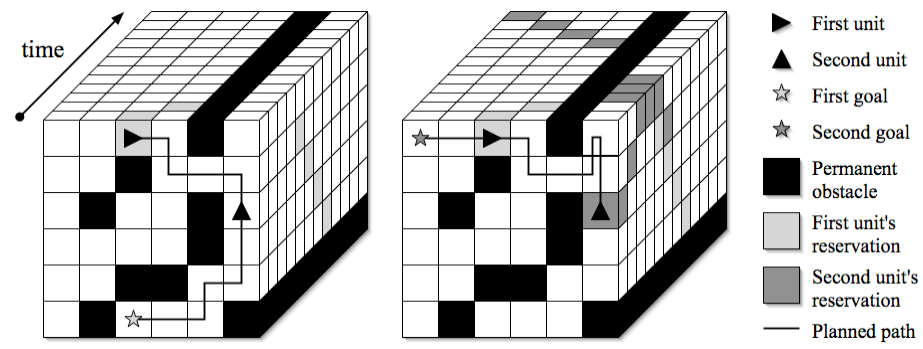
\includegraphics[width=10cm]{img/reservation-table}
	\caption{Dwie jednostki kooperacyjnie poszukujące tras. (A) Pierwsza jednostka znajduje ścieżkę i zaznacza ją w tablicy rezerwacji. (B) Druga jednostka znajduje ścieżkę, uwzględniając istniejące rezerwacje pól, również zaznaczając ją w tablicy rezerwacji. Źródło: \cite{cooppath}}
	\label{fig:img_reservation-table}
\end{figure}

W ogólności poszczególni agenci mogą mieć różną prędkość lub rozmiary, zatem tablica rezerwacji musi mieć możliwość zaznaczenia dowolnego zajętego obszaru. Zostało to przedstawione na rysunku \ref{fig:img_reservation-table-2}.

\begin{figure}[H]
	\centering
	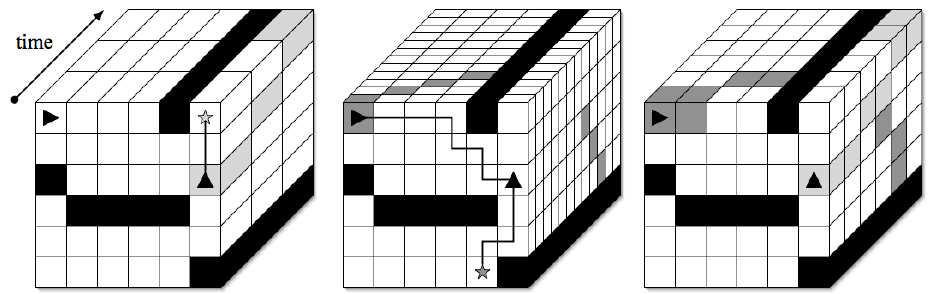
\includegraphics[width=10cm]{img/reservation-table-2}
	\caption{Czasoprzestrzenna mapa może różnić się od tablicy rezerwacji. (A) Powolna jednostka ma "głębokie" komórki na czasoprzestrzennej mapie. (B) Szybka jednostka ma "płytkie" komórki. (C) Tablica rezerwacji jest współdzielona między wszystkimi agentami, dlatego powinna być odpowiednio dopasowana do wszystkich agentów. Źródło: \cite{cooppath}}
	\label{fig:img_reservation-table-2}
\end{figure}

Jeśli tylko mała część z całej tablicy rezerwacji będzie markowana jako zajęta, wydajniej jest zaimplementować ją jako tablicę typu {\it hash table}. Daje to zaletę oszczędności pamięci poprzez pamiętanie jedynie współrzędnych $(x, y, t)$ zajętych pól.

Niestety taki sposób wykorzystania tablicy rezerwacji w pewnych sytuacjach nie zapobiega zderzeniom czołowym jednostek zmierzających w przeciwnych kierunkach.
Jeśli jedna jednostka zarezerwowała komórki $(x, y, t)$ i $(x + 1, y, t + 1)$, nic nie stoi na przeszkodzie, aby kolejna jednostka mogła zarezerwować komórki $(x + 1, y, t)$ i $(x, y, t + 1)$. Ten problem może być rozwiązany poprzez zajmowanie (rezerwowanie) dwóch sąsiednich komórek w tym samym czasie $t$ podczas ruchu robota.

\section{Hierarchical Cooperative A*}
\label{ch:hier_cooperative_a}
$TODO$
The second generic method for improving a heuristic based on abstractions of the state space is to use Hierarchical A*.
With this approach the abstract distances are computed on demand. The hierarchy in this case refers to a
series of abstractions of the state space, each more general
than the previous, and is not restricted to spatial hierarchy.
The choice of hierarchy is critical, and that
large hierarchies may in fact perform worse than small, sim-
ple hierarchies.

Hierarchical Cooperative A* (HCA*) uses a simple hier-
archy containing a single domain abstraction, which ignores
both the time dimension and the reservation table. In other
words, the abstraction is a simple 2-dimensional map with
all agents removed. Abstract distances can thus be viewed
as perfect estimates of the distance to the destination, ig-
noring any potential interactions with other agents. This is
clearly an admissible and consistent heuristic. Furthermore,
the inaccuracy of the heuristic is determined only by the dif-
ficulty of interacting with other agents (how much the agent
must deviate from the direct path to avoid other agents).

A fourth approach is introduced here, which is to use a Reverse
Resumable A* (RRA*) search in the abstract domain.
The RRA* algorithm executes a modified A* search in a
reverse direction. The search starts at the agent’s goal G,
and heads towards the agent’s initial position O. Instead
of terminating at O, the search continues until a specified
node N is expanded.

HCA* is just like CA* with a more sophisticated heuris-
tic, using RRA* to calculate the abstract distance on demand.
\cite{cooppath}

\section{Windowed Hierarchical Cooperative A*}
$TODO$
One issue with the previous algorithms is how they termi-
nate once the agents reach their destination. If an agent sits
on its destination, for example in a narrow corridor, then
it may block off parts of the map to other agents. Ideally,
agents should continue to cooperate after reaching their des-
tinations, so that an agent can move off its destination and
allow others to pass.

A second issue is the sensitivity to agent ordering. Al-
though it is sometimes possible to prioritise agents globally
(Latombe 1991), a more robust solution is to dynamically
vary the agent order, so that every agent will have the high-
est priority for a short period of time. Solutions can then
be found which would be unsolvable with an arbitrary, fixed
agent order.

A simple solution to all of these issues is to window the
search. The cooperative search is limited to a fixed depth
specified by the current window. Each agent searches for a
partial route to its destination, and then begins following the
route. At regular intervals (e.g. when an agent is half-way
through its partial route) the window is shifted forwards and
a new partial route is computed.

To ensure that the agent heads in the correct direction,
only the cooperative search depth is limited to a fixed depth,
whilst the abstract search is executed to full depth. A win-
dow of size w can be viewed as an intermediate abstraction
that is equivalent to the base level state space for w steps,
and then equivalent to the abstract level state space for the
remainder of the search. In other words, other agents are
only considered for w steps (via the reservation table) and
are ignored for the remainder of the search.
\cite{cooppath}


$TODO$
One example of a decoupled approach is HCA* [Silver,
2005]. HCA* employs a reservation table for timestep-
location pairs. The algorithm chooses a fixed ordering of
agents, and plans a path for each agent in turn that avoids con-
flicts with previously computed paths by checking against the
reservation table. Unfortunately, in over half of our bench-
mark instances, some agents never reach their destinations
because the paths found for previous agents in the fixed or-
der can make finding paths for subsequent agents impossi-
ble. Using a windowed search, Silver’s WHCA* mitigates
this problem at the cost of solution quality and running time.
\cite{completealgo_standley}

$TODO$
WHCA* (Windowed Hierarchical Cooperative A*) uses a temporal-spatial search, that
is, a node in the search tree is not only defined by the position, but is also defined by the
time the agent will be there. The search is also windowed; this means that it is performed
a fixed number of steps into the future, and the most promising node at the edge of this
window is selected.
To plan all the agents' paths at the same time carries an all-to-high computational cost[9].
Instead, a reservation table is used. The path of every agent is planned independently, and
every position and time that a node is blocked is recorded in the reservation table. This is
a reasonable approach to decrease the computational costs involved, which although it may
not solve all problems, will be able to solve many of them.
To focus the search, a spatial reverse A* search is used as heuristic for the temporal-
spatial search. That is, it is used to calculate the exact distance from a node to the goal,
excluding the influence other agents may have on this distance. This generally focuses the
search a lot, as this is often a very high-quality heuristic. It gets worse with a higher level
of congestion in the environment.
However, this reverse A* search leads to a high initial cost when performing the first
windowed temporal-spatial search, as it needs to perform a full A* search from the goal
to the start (as well as to some nodes neighbouring the start), but the cost for subsequent
searches will be lower.
\cite{rtcooppathfinding}

Windowed Hierarchical Cooperative A*:
• Cooperative A*
• Hierarchical Heuristic
• Windowed cooperation

Use a hash table to store time-space indexed reservations
• Reserve / Free a space/time cell

$TODO$ Clearance-based Pathfinding and Hierarchical Annotated A* Search - używane, gdy jednostki zajmują różne obszary, ale chyba tylko dla jednej jednostki (nie cooperative)
\clearpage{\pagestyle{empty}\cleardoublepage}

\chapter{Podsumowanie}
\label{ch:podsumowanie}

$TODO$
Większość algorytmów Cooperative Pathfinding opiera się o A*

Algorytmy wprowadzają ograniczenie (błędne założenie), że ruchy trwają tyle samo. Można robić inaczej: podzielić dyskretnie i zaznaczać zajętość pól w wielu kratkach - ale wtedy będzie więcej obliczeń.

Windowed Hierarchical Cooperative A*:
• Cooperative A*
• Hierarchical Heuristic
• Windowed cooperation

The cooperative pathfinding methods are more successful
and find higher quality routes than A* with Local Repair.
Unfortunately, the basic CA* algorithm is costly to compute,

The size of the window has a significant effect on the suc-
cess and performance of the algorithm. With a large win-
dow, WHCA* behaves more like HCA* and the initialisa-
tion time increases. If the window is small, WHCA* be-
haves more like Local Repair A*. The success rate goes
down and the path length increases. The window size pa-
rameter thus provides a spectrum between Local Repair A*
and HCA*. An intermediate choice appears to give the most robust overall performance.
In general, the window size should be set to the duration
of the longest predicted bottleneck. In Real-Time Strategy
games groups of units are often moved together towards a
common destination. In this case the maximum bottleneck
time with cooperative pathfinding (ignoring units in other
groups) is the number of units in the group. If the window
size is lower than this threshold, bottleneck situations may
not be resolved well. If the window size is higher, then some
redundant search will be performed.

Local Repair A* may be an adequate solution for simple en-
vironments with few bottlenecks and few agents. With more
difficult environments, Local Repair A* is inadequate and is
significantly outperformed by Cooperative A* algorithms.

By introducing Hierarchical A* to improve the heuristic and
using windowing to shorten the search, a robust and efficient
algorithm, WHCA*, was developed. WHCA* finds more
successful routes than Local Repair A*, with shorter paths
and fewer cycles.

Although this research was restricted to grid environ-
ments, the algorithms presented here apply equally to more
general pathfinding domains. Any continuous environment
or navigational mesh can be used, so long as each agent’s
route can be planned by discrete motion elements. The grid-
based reservation table is generally applicable, but reserving
mesh intersections may be more appropriate in some cases.
Finally, the cooperative algorithms may be applied in dy-
namic environments, so long as an agent’s route is recom-
puted whenever invalidated by a change to the map.


Cooperative pathfinding is a general technique for coordinating the paths of many units.
It is appropriate whenever there are many units on the same side who are able to
communicate their paths. By planning ahead in time as well as space, units can get out of
each other’s way and avoid any conflicting routes.

Many of the usual enhancements to spatial A* can also be applied to space-time A*.
Moreover, the time dimension gives a whole new set of opportunities for pathfinding
algorithms to explore.

\clearpage{\pagestyle{empty}\cleardoublepage}

\phantomsection
\addcontentsline{toc}{chapter}{Bibliografia}
\bibliographystyle{unsrt}	
\bibliography{bibliography}
\clearpage

\phantomsection
\addcontentsline{toc}{chapter}{Wykaz skrótów}
\chapter*{Wykaz skrótów}

\begin{tabular}{l l}
API & Application Programming Interface \\
SDK & Software Development Kit \\


\end{tabular}

\clearpage

\phantomsection
\addcontentsline{toc}{chapter}{Spis rysunków}
\listoffigures
\clearpage

% \phantomsection
% \addcontentsline{toc}{chapter}{Spis tabel}
% \listoftables
% \clearpage